\section[Maven]{Maven}
\subsection[]{Introduction}
\begin{frame}
\frametitle{Building java applications}
\begin{itemize}
	\item Motivation aka \emph{Why should we care, let's have bash script with bunch of javac commands}
	\item Brief look into history
		\begin{itemize}
		\item Make % 1977
		\item Ant (with Ivy) %XML - 2000
		\item Maven %XML  - 2005
		\item Gradle %DSL based on Groovy (used by google to build Android), less boilerplate - 2012
		\end{itemize}
\end{itemize}
\end{frame}

% Ant
%    -  XML, procedural, scripting tool, originally intended to replace make
%    - nothing is standardized (clean vs clear)
%    - need to explicitely do everything
%    - easier to learn than maven (but is really just a scripting tool)

\begin{frame}
\frametitle{Build tools - history overview}
	\begin{center}
		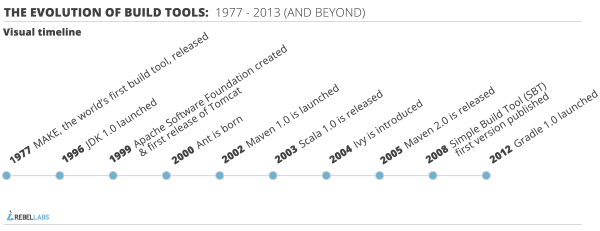
\includegraphics[width=\textwidth,height=0.385\textwidth]{build-tools-history.png}
	\end{center}
\end{frame}

\begin{frame}
\frametitle{Build tools - popularity}
	\begin{center}
		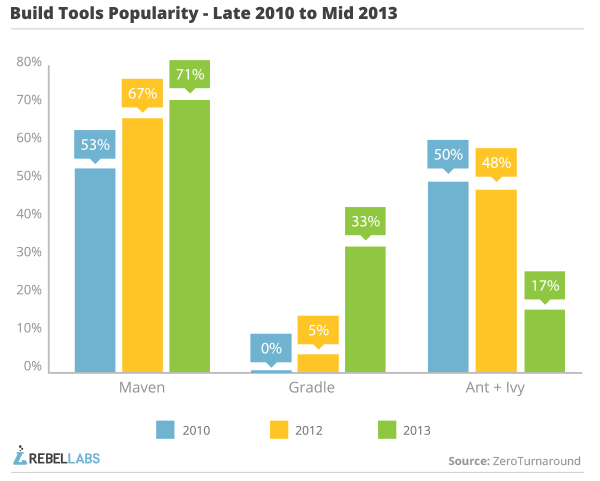
\includegraphics[width=0.8\textwidth,height=0.64\textwidth]{build-tools-popularity.png}
	\end{center}
\end{frame}

\begin{frame}
\frametitle{Desired properties of quality build tool}
\begin{itemize}
	\item How steep is learning curve
	\item Time required for build
	\item Complexity of build script (creation, maintenance)
	\item Extensibility and flexibility (plugins)
	\item Build environment consistency
	\item Extra features (docs, deployment, etc...)
	\item Integration with developer tools (IDEs, CI servers,...)
\end{itemize}
\end{frame}

\begin{frame}
\frametitle{Maven basics}
\begin{itemize}
	\item Software project management and comprehension tool %help to comprehend/understand any java-based project
		\begin{itemize}
		\item Describes how software project is built
		\item Describes software project dependencies
		\end{itemize}
	\item Developed by Apache Software Foundation
	\item Created 2004, current version 3.5.0 (Apr 2017)
	\item Written in Java
	\item XML configured
\end{itemize}
\end{frame}

\begin{frame}
\frametitle{Maven characteristics}
\begin{itemize}
	\item Consistency across projects, standardized build environment
	\item Lot of implicit functionality (mvn clean is standardized)
	\item Inheritance via parent poms
	\item Dependency management, transitive dependencies
	\item Convention over configuration
		\begin{itemize}
		\item If mvn conventions are followed then it's easy, if not, it can become very complicated
		\end{itemize}
	\item Centered around managing entire projects lifecycle
\end{itemize}
\end{frame}

\begin{frame}
\frametitle{Maven - POM file}
\begin{itemize}
	\item XML definition of a project
	\item Defines:
		\begin{itemize}
		\item Project information 
			\begin{itemize}
			\item Name
			\item Company allegiance
			\item Docs
			\item Test coverage
			\item Version
			\end{itemize}
		\item Parent relation
		\item Dependencies
		\item Plugins to be used
		\item Build steps
		\end{itemize}
\end{itemize}
\end{frame}

\begin{frame}
\frametitle{Maven - Features}
\begin{itemize}
	\item Dependency management
		\begin{itemize}
		\item Scope
			\begin{itemize}
			\item compile (default)
			\item provided
			\item test
			\end{itemize}
		\item Library versions
		\end{itemize}
	\item Versioning
		\begin{itemize}
		\item SNAPSHOTs
		\item Deployment of stable versions into repository
			\begin{itemize}
			\item Central Maven repository
			\item Company proxy - Artifactory, Nexus
			\end{itemize}
		\end{itemize}		
\end{itemize}
\end{frame}

\begin{frame}
\frametitle{Maven - Features}
\begin{itemize}
	\item Packaging
		\begin{itemize}
		\item jar (default)
		\item war
		\item ear
   		\item pom
		\end{itemize}
	\item Archetypes
		\begin{itemize}
		\item Ability to quickly setup template projects
		\item Way of standardization of company guidelines and frequently used patterns
		\end{itemize}			
\end{itemize}
\end{frame}

\begin{frame}
\frametitle{Maven - Plugins}
\begin{itemize}
	\item Standardized shared functionality execution
	\item All work in Maven is done by plugins
	\item Build plugins (project consolidation)
	\item Reporting plugins (tests, site, docs)
	\item Each plugin can have several goals (e.g. \textbf{mvn jetty:run})
	\item Standard plugins \url{https://maven.apache.org/plugins/}
		\begin{itemize}
		\item \textbf{mvn clean}
		\item \textbf{mvn package}
  		\item \textbf{mvn install}
  		\item \textbf{mvn deploy}
		\end{itemize}	
\end{itemize}
\end{frame}

\begin{frame}
\frametitle{Maven - Lifecycle}
\begin{itemize}
	\item Clearly defined process for project build and distribution
	\item Consisting of phases
		\begin{itemize}
		\item Phase consists of plugin goals
		\end{itemize}
	\item 3 built-in lifecycles
		\begin{itemize}
		\item default (validate, compile, test, package, verify, install, deploy)
			\begin{itemize}
			\item Each phase triggers all previous (eg. mvn test executes validate and compile before test)
			\end{itemize}
		\item clean
		\item site
		\end{itemize}
	\item Customizable (defining own lifecycles)
\end{itemize}
\end{frame}

\begin{frame}
\frametitle{Maven - Best practices}
\begin{itemize}
	\item Single artifact per pom.xml
	\item Using POM recommended layouts - \href{https://maven.apache.org/pom.html}{ref}
	\item Versions for plugins and dependencies to be kept in parent mgmt section
	\item Put all artifacts into target folder (follow conventions)
	\item Use dependency plugin to analyze goals to identify issues
	\item Follow conventions (e.g. directory structure - \href{https://maven.apache.org/guides/introduction/introduction-to-the-standard-directory-layout.html}{ref})
	\item Do not make Maven act like Ant
\end{itemize}
\end{frame}

\subsection[]{Maven - Demo}
\begin{frame}
\frametitle{Maven - Demo}
% POM example
% basic lifecycle/commands
% archetypes
\end{frame}








